\documentclass[titlepage, letterpaper, 10.5pt]{article}
\usepackage[letterpaper, margin=1.25in]{geometry}
\usepackage{graphicx}
\usepackage{comment}
\usepackage{amsmath}
\usepackage{caption}
\usepackage{subcaption}
\usepackage{nicefrac}
\usepackage{tablefootnote}
\begin{document}

\title{Emitter-Coupled Oscillator}
\author{Author: Ben Lorenzetti}
\date{Project Start Date: February 26, 2015\\
Report Submission Date: March 23, 2015}
\maketitle

\clearpage
\mbox{}
\thispagestyle{empty}
\clearpage
\setcounter{page}{1}

\tableofcontents

\section{Objective}

To investigate the design and operation of an emitter-coupled astable multivibrator for 50
MHz operation.

\clearpage
\section{Principles of Operation}

In analog electronics, a sinusoidal oscillator is sometimes needed,
such as for power conversion, driving a motor, or for the carrier frequency in radio transmissions.
These can be built from an amplifier with a passive feedback network,
where the $\textrm{gain}>1$ and the feedback is positive at the frequency of operation
\footnote{the Barkhausen Criterion}.
The only other requirement is that the amplifer operates linearly.

In contrast, digital circuits usually require a square wave clock signal.
Ironically, a digital oscillator can be built starting from a basic digital component.

A latch is a digital circuit with two stable states, made from two cross-connected amplifiers.
It is a fundamental component in digital logic.
In fact, when a master and slave latch are connected in series they form a 1-bit, flip-flop register used in CPUs.
Usually, the cross-connection between the two amplifiers is resistive and one amplifier
will be driven in saturation while the other is in cutoff.
Amplifier in digital circuits are usually driven between saturation and cutoff,
making them unlinear, binary (two-state) devices.

\begin{figure}[ht]
	\centering
	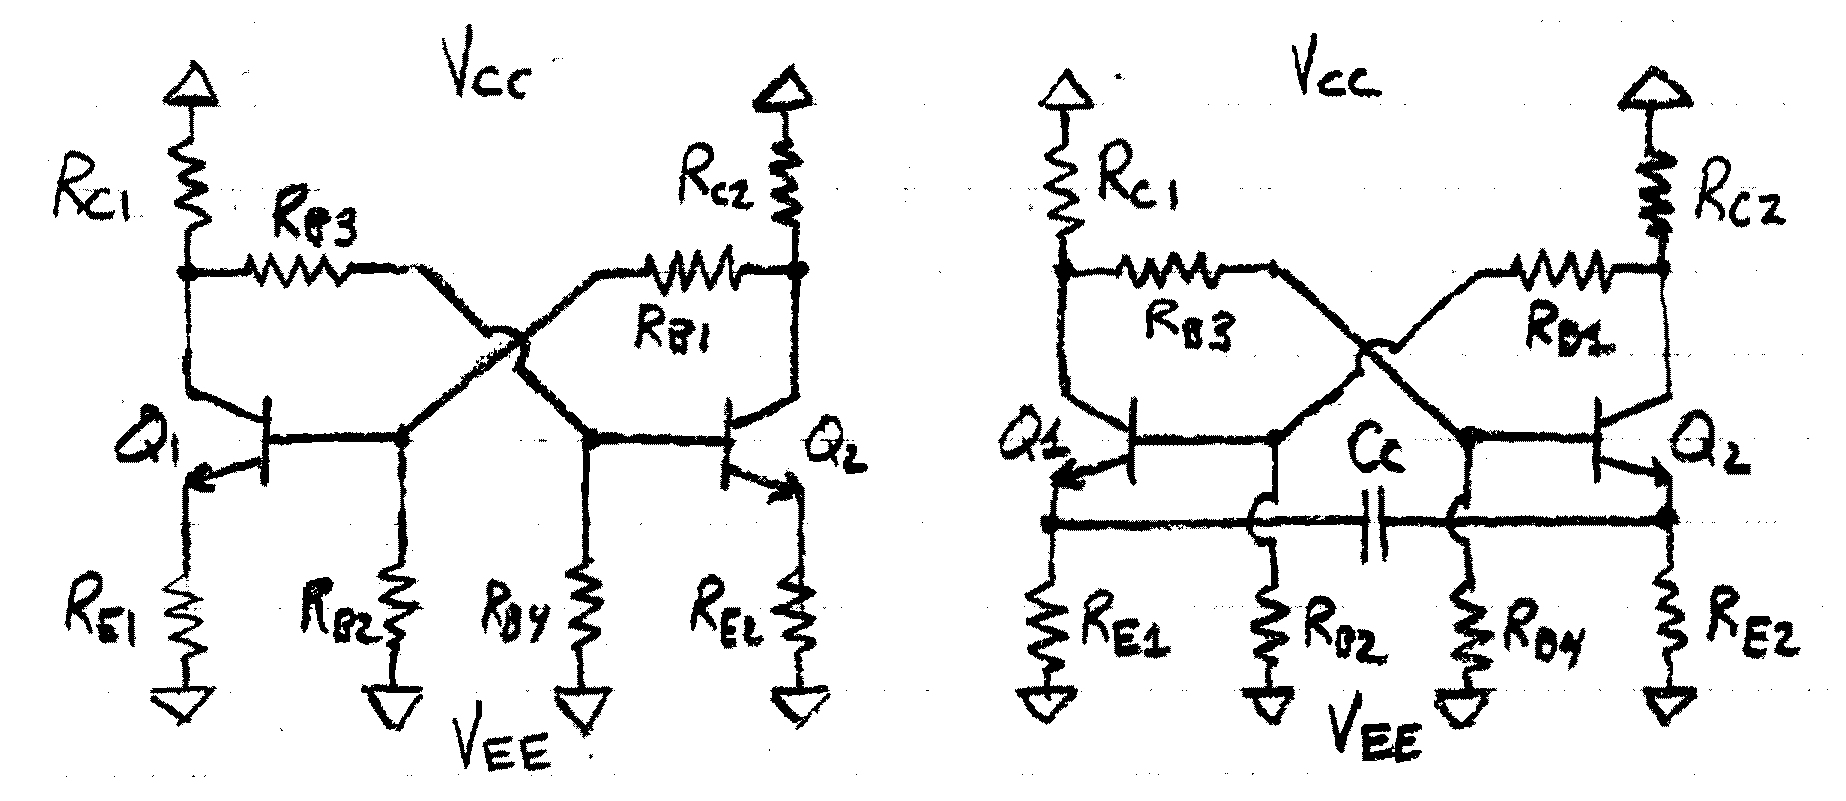
\includegraphics[width=0.6\textwidth]{diagrams/latches.png}
	\caption{Digial Latch (left) and Latch with Reactive Emitter Coupling (right).}
	\label{latches}
\end{figure}

If the cross-connection is made to be reactive, then the latch may not be stable in either state.
If it oscillates between the two states and produces a near-square wave, it is called a bistable multivibrator.
A capacitor is usually used for the cross-connection because it delays the instantaneous voltage change
that would normally occur when a transistor switches between saturation and cutoff.

Analog oscillators produce sinusoids; digital oscillators produce square waves.
An analog amplifer oscillates if it has reactive feedback that is positive;
a digital flip-flop oscillates if it has reactive cross-connection strong enough to switch states.
Analog oscillators use an amplifier in a linear range; digital oscillators use drive
amplifier to its two limits.
An analog oscillator may form unintentionally through parasitic feedback,
such as through the Miller capacitance of a BJT.
A digital osciallator may form unintentionally through propagation delay or carry-through
logic
All of these comparisons between analog and digital oscillators can probably be gleaned
from the block-level diagrams in figure \ref{oscillator-block-diagrams}.

\begin{figure}[ht]
	\centering
	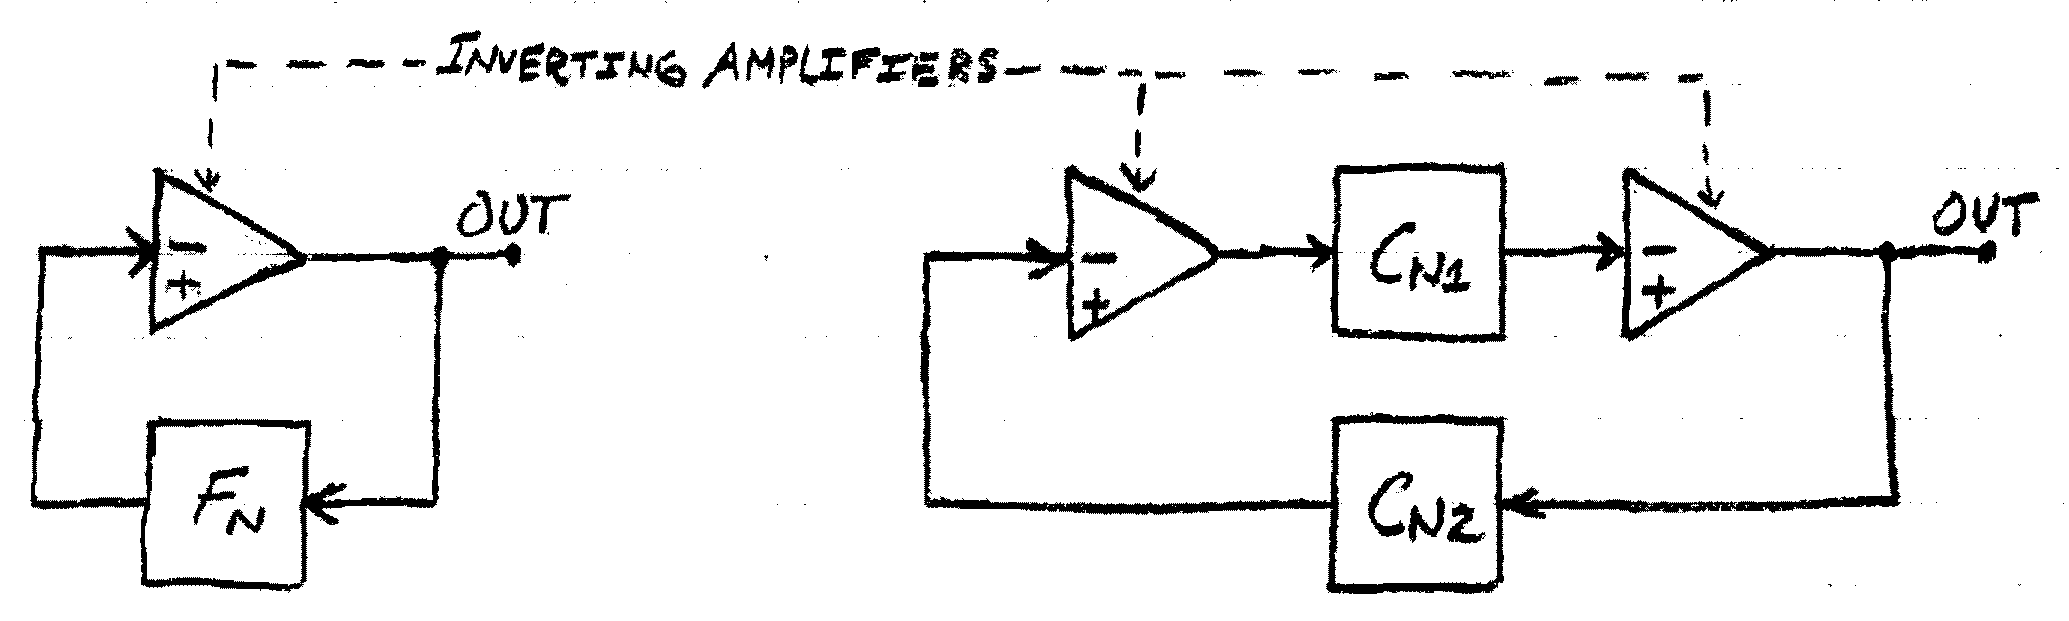
\includegraphics[width=0.7\textwidth]{diagrams/block-level-oscillators}
	\caption{An Analog Feedback Oscillator (left) Compared to Bistable Multivibrator (right)}
	\label{oscillator-block-diagrams}
\end{figure}

\clearpage
\section{Theory}

\subsection{Bistable Latch}
\label{bistable-latch}

A digital latch can be built with two cross-connected BJT amplifiers, shown in figure
\ref{latch-circuit-diagram}. The amplifiers should be nearly mirror images of one another and the
coupling networks should be entirely resistive.

\begin{figure}[ht]
	\centering
	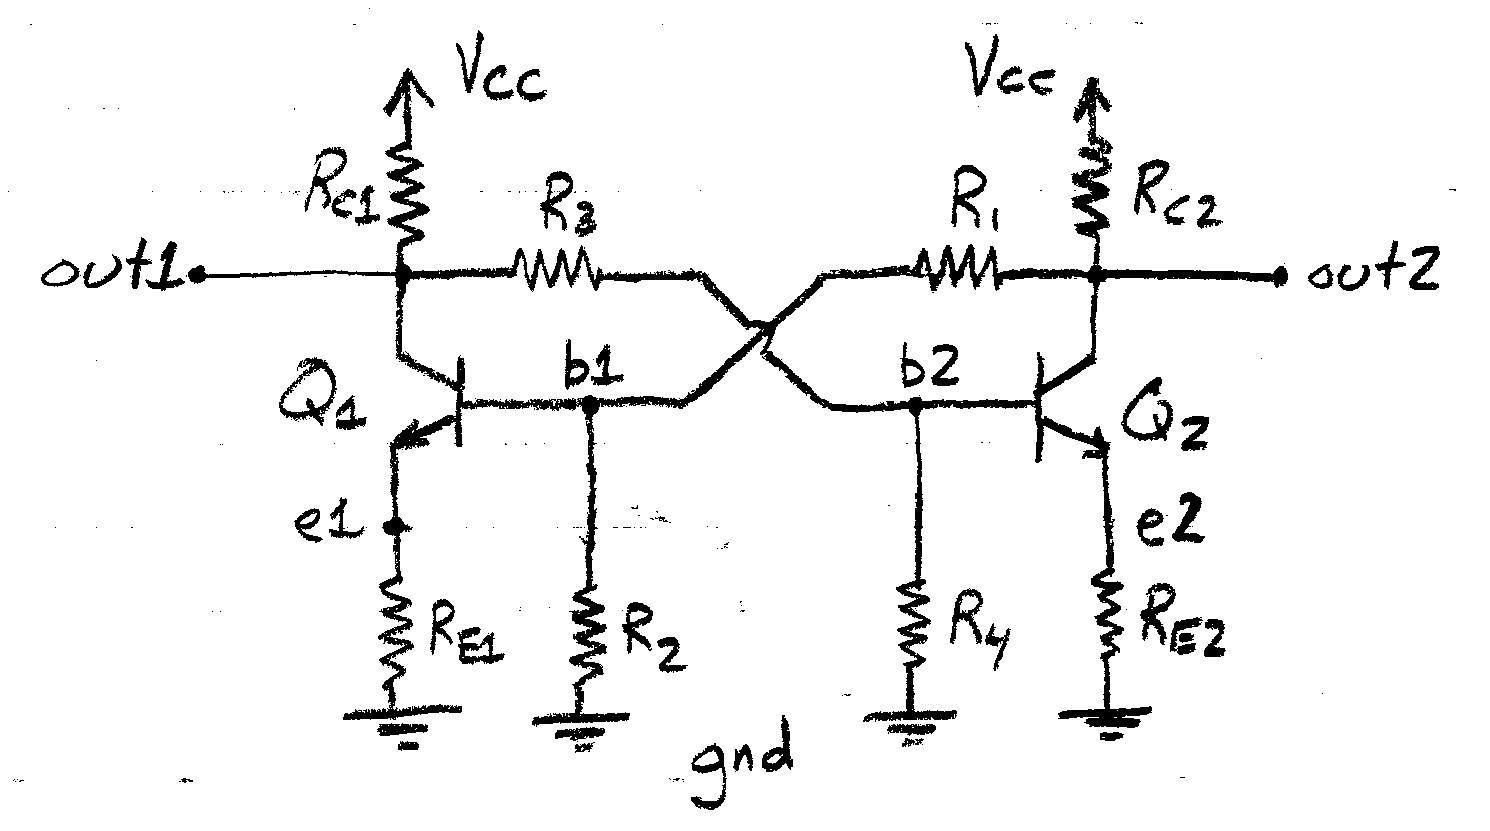
\includegraphics[width=0.6\textwidth]{diagrams/latch-circuit}
	\caption{BJT Implementation of a Digital Latch}
	\label{latch-circuit-diagram}
\end{figure}

The latch is bistable, meaning it has two self-sustaining states.
Either Q1 is saturated while Q2 is cutoff, or Q1 is cutoff while Q2 is saturated.
The circuit is a symmetric loop, so it is not clear where to begin any analysis.
Instead of starting at a particular node and time, we will start with some sanity
assumptions and determining the conditions that make them true.

If the transistors operate digitally--i.e. either in saturation or cutoff--then the output
can have two possible values, the difference between which will be called $V_{pkpk}$.
This difference is set by $R_{C}$ and the saturation current.
\begin{equation}
R_{C}=\frac{V_{pkpk}}{I_{C(sat)}}
\label{rc-eq}
\end{equation}

Of course, this assumes that the current through $R_{1}$ and $R_{2}$ is negligible compared to $I_{C(sat)}$.
\begin{equation*}
I_{Bias}<<I_{C(sat)}
\end{equation*}

Another design assumption is the stiff base bias.
In order to stiffly bias the transistors, the base currents should draw negligible current
relative to $R_{1}$ and $R_{2}$.
\begin{equation*}
I_{B(sat)}<<I_{Bias}
\end{equation*}

These two biasing network equations
compete with each other because the base and collector currents are related by $\beta$.
The best way to satisfy both is
\begin{equation}
I_{Bias}=\frac{I_{C(sat)}}{\sqrt{\beta}}
\label{i-bias-design-decision}
\end{equation}

If the supply voltage is relatively large compared to the output amplitude,
then $I_{Bias}$ varies little with binary state and is set by $R_{1}$ and $R_{2}$.
\begin{equation}
I_{Bias}=\frac{V_{CC}}{R_{1}+R_{2}}
\label{i-bias-eq}
\end{equation}

Combining equations \ref{i-bias-design-decision} and \ref{i-bias-eq} helps in designing
the bias network.
\begin{equation}
R_{1}+R_{2}=\frac{\sqrt{\beta}V_{CC}}{I_{C(sat)}}
\label{r1r2-eq}
\end{equation}

The analysis so far has assumed that the saturation current is fixed,
but should it be fixed with $R_{C}$ or $R_{E}$?
It makes more sense to limit $I_{C(sat)}$ with $R_{C}$ because
later we will be adding a reactive element to the emitters.

For the transistor to be driven to saturation, $V_{CE}$ is approximately equal to $V_{BE(on)}$
and the collector is equipotential with the base. The collector potential
during saturation is the lesser of the two binary outputs, so
\begin{equation}
V_{B(sat)}=V_{CC}-V_{pkpk}
\label{saturation-condition}
\end{equation}

For the other transistor to be cutoff,
the base-emitter junction must not have achieved the forward bias potential.
\begin{equation}
V_{B(off)}<V_{E(off)}-V_{BE(on)}
\label{cutoff-condition}
\end{equation}

The transistors are cross-connected from their outputs to the opposite bases, so the base bias
is dependent on the opposite transistor's state. The bias networks are voltage dividers and the output
has two states, so the base potential is one of the two following values.
\begin{equation}
V_{B}=
\left\{
	\begin{array}{lr}
	\frac{R_{2}}{R_{1}+R_{2}}V_{CC}	& : \textrm{saturation transistor}	\\
	\frac{R_{2}}{R_{1}+R_{2}}(V_{CC}-V_{pkpk})	& : \textrm{cutoff transistor}
	\end{array}
\right.
\label{base-voltages}
\end{equation}

Combining the required conditions for saturation and cutoff from equations
\ref{saturation-condition} and \ref{cutoff-condition}
with the two biasing potentials gives the conditions for stability of the latch.
\begin{equation*}
\left\{
	\begin{array}{lr}
	\frac{R_{2}}{R_{1}+R_{2}}V_{CC}=V_{CC}-V_{pkpk}	& : \textrm{saturation stability}	\\
	\frac{R_{2}}{R_{1}+R_{2}}(V_{CC}-V_{pk-pk})<V_{E(off)}+V_{BE(on)}	& : \textrm{cutoff stability}
	\end{array}
\right.
\end{equation*}

A latch is only useful if the output is self-sustaining, so these two conditions must both be met.
The first condition has all fixed values, so the ratio $\nicefrac{R_{2}}{R_{1}+R_{2}}$ must be chosen there.
The second condition can then be rearranged to separate fixed values from as-yet-undetermined values.
\begin{equation}
\left\{
	\begin{array}{lr}
	\frac{R_{2}}{R_{1}+R_{2}}=\frac{V_{CC}-V_{pkpk}}{V_{CC}}	& : \textrm{saturation stability}	\\
	V_{E(off)}>\frac{R_{2}}{R_{1}+R_{2}}(V_{CC}-V_{pkpk})-V_{BE(on)}	& : \textrm{cutoff stability}
	\end{array}
\right.
\label{stability-conditions}
\end{equation}

The stability conditions for both transistors would have to be followed if we were
designing digital memory. However, for an oscillator we only want quasi-stable states;
in the next section we will violate the stability by adding reative coupling to affect $V_{E}$ of the off transistor.

\clearpage
\subsection{Astable Multivibrator}
\label{astable-multivibrator}

The simple circuit for an astable multivibrator is shown in figure \ref{simple-circuit-diagram}.
Topologically it is easy to make--just add a capactitor to a BJT latch.

\begin{figure}[ht]
	\centering
	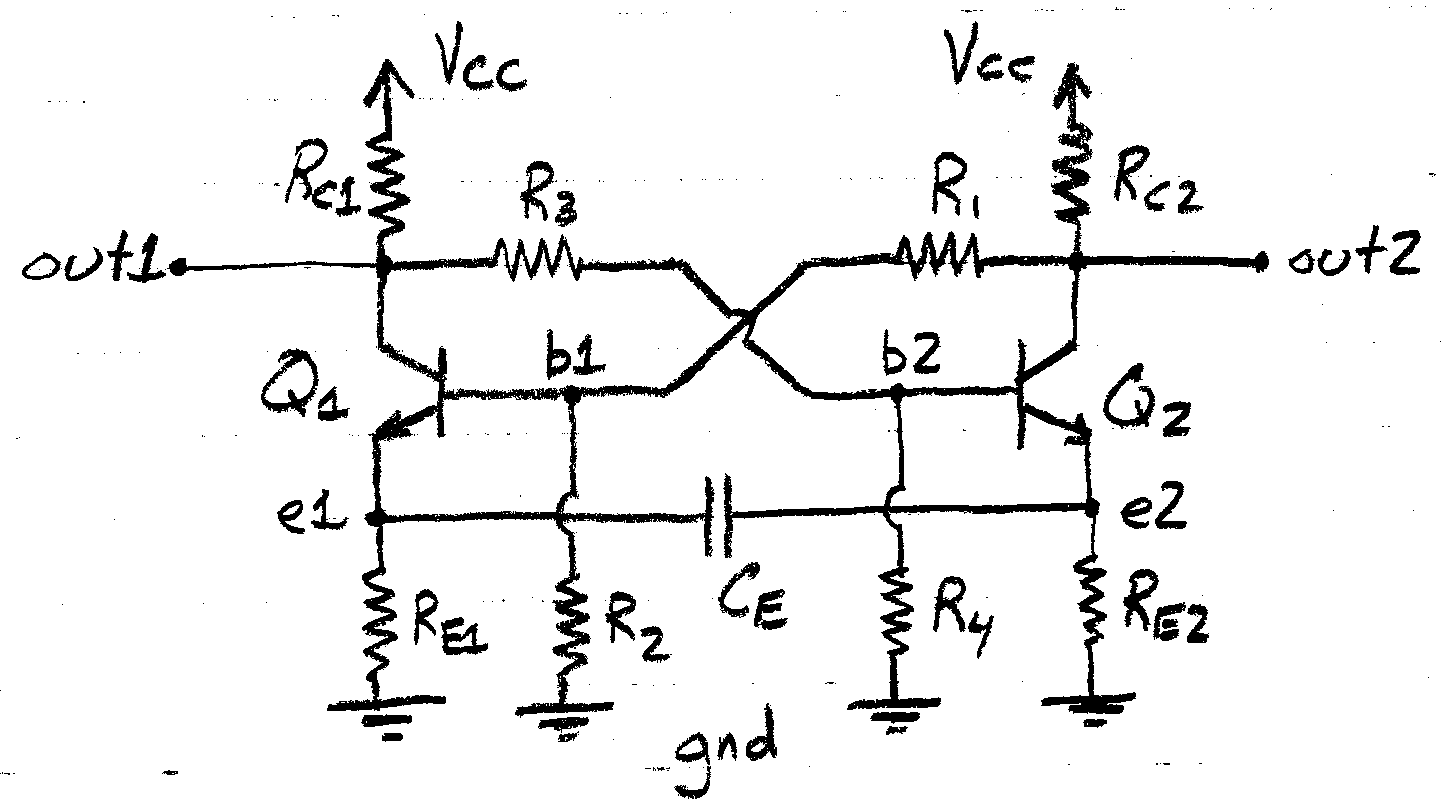
\includegraphics[width=0.6\textwidth]{diagrams/simple-circuit}
	\caption{Simple Version of Astable Multivibrator}
	\label{simple-circuit-diagram}
\end{figure}

The top half of the circuit is the same as the latch.
The relationships between $I_{C(sat)}$ and $V_{pkpk}$ to $R_{C}$, $R_{1}$, and $R_{2}$
is the same as in equations \ref{rc-eq} through \ref{stability-conditions}.
Now for the bottom half.

The emitter potential for the saturation transistor is set by the top half because
it follow the base. Taking the saturation base voltage from equation \ref{base-voltages}...
\begin{equation}
V_{E(sat)}=\frac{R_{2}}{R_{1}+R_{2}}V_{CC}-V_{BE(on)}
\label{ve-sat-eq}
\end{equation}

In a perfect world,
this emitter voltage would hold regardless of $R_{E}$.\footnote{Actually in a perfect world, I would have already graduated.}
However, in the interest of not burning up the base-emitter junction, $R_{E}$
should probably be just short of becoming the saturation current limiter.
\begin{equation}
R_{E}=\frac{V_{E(sat)}}{I_{E(sat)}}=\frac{\frac{R_{2}}{R_{1}+R_{2}}V_{CC}-V_{BE(on)}}{I_{C(sat)}}
\label{re-eq}
\end{equation}

Equation \ref{stability-conditions} described the stability conditions for the latch.
To make an oscillator, the circuit should be quasistable--i.e. it should be stable for some
specific length of time. After a period of stable output, an internal trigger cause a change of state.
For the emitter-coupled oscillator, the trigger is the emitter potential of the cutoff transistor
falling below $V_{E(off)}$. From equation \ref{stability-conditions}, the cutoff state is stable while
\begin{equation*}
V_{E(off)}>\frac{R_{2}}{R_{1}+R_{2}}(V_{CC}-V_{pkpk})-V_{BE(on)}
\end{equation*}

The capacitor prevents instantaneous voltage changes, so it takes some time for $V_{E}$
to fall below this trigger threshold. We expect an RC time constant for the discharge to be on
order of $\tau=R_{E}C_{E}$, but solving for the transient equation may give additional insights.
\begin{equation*}
i(t)=C\frac{dv(t)}{dt} \quad \quad \textrm{resists instantaneous } \delta V
\end{equation*}

The cross-connected bases make the transistors behave somewhat like a emitter-follower voltage source.
If we assume that switching times for the transistors is negligible, then the transient circuit
is as shown in figure \ref{simple-transient-circuit}. This assumption is true if the base-emitter
capacitance is negligible, and so is the delay in the BJT due to the rate of minority carrier diffusion.

\begin{figure}[ht]
	\centering
	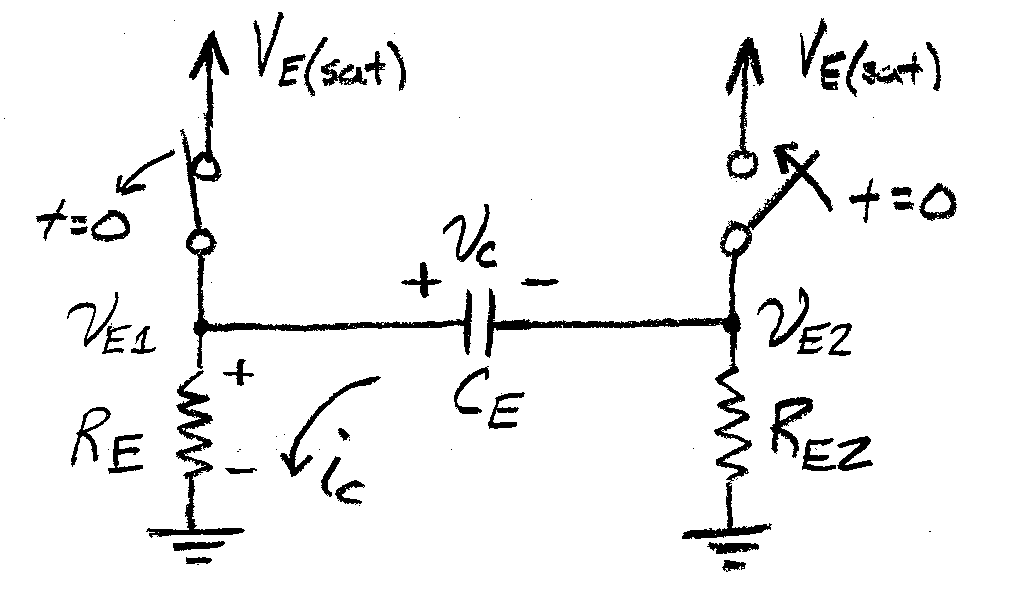
\includegraphics[width=0.45\textwidth]{diagrams/simple-transient-circuit}
	\caption{Transient Circuit for Simple Emitter-Coupled Oscillator}
	\label{simple-transient-circuit}
\end{figure}

At t=0, $Q_{2}$ triggers itself on by $v_{E2}$ falling below the threshold.
In turn, this forces $Q_{1}$ off through the cross connection.
This trigger occurs when $v_{E2(off)}$ breaks the stability condition.
\begin{equation}
V_{E(trig)}=\frac{R_{2}}{R_{1}+R_{2}}(V_{CC}-V_{pkpk})-V_{BE(on)}
\label{ve-trig-eq}
\end{equation}

Immediately before the trigger occurs, the voltage at E1 is $V_{E(sat)}$ and
the voltage at E2 is the trigger voltage $V_{E(trig)}$.
So, the initial voltage across the capacitor is
\begin{equation}
v_{C}(0^{-})=V_{E(sat)}-V_{E(trig)}
\end{equation}

With the initial conditions in hand, we are ready to analyze the transient circuit.
After switching, $R_{E2}$ does not matter because $Q_{2}$ acts like a voltage source.
Consequently there is only one loop to analyze: the $v_{E1}$ discharge loop.
The differential equation describing the loop is found from Kirchoff's Voltage Law.
\begin{equation}
v_{E1}(t):=\quad R_{E}i_{C}(t)=V_{E(sat)}u(t)+v_{C}(t)
\label{ve1-kvl}
\end{equation}

\begin{equation*}
R_{E}\left(-C_{E}\frac{dv_{C}(t)}{dt}\right)=V_{E(sat)}u(t)+v_{C}(t)
\end{equation*}

\begin{equation}
\frac{d}{dt}v_{C}(t)+\frac{1}{R_{E}C_{E}}v_{C}(t)=\frac{-V_{E(sat)}}{R_{E}C_{E}}u(t)
\end{equation}

The system will be easier to solve in frequency domain. Taking the Laplace transform gives
\begin{equation*}
sV_{C}(s)-v_{C}(0^{-})+\frac{1}{R_{E}C_{E}}V_{C}(s)=\frac{-V_{E(sat)}}{sR_{E}C_{E}}
\end{equation*}

\begin{equation*}
V_{C}(s)\left[s^{2}+\frac{s}{R_{E}C_{E}}\right]=
sv_{C}(0^{-})-\frac{V_{E(sat)}}{R_{E}C_{E}}
\end{equation*}

\begin{equation*}
V_{C}(s)=\frac{sv_{C}(0^{-})-\frac{V_{E(sat)}}{R_{E}C_{E}}}
{s(s+\frac{1}{R_{E}C_{E})}}
\end{equation*}

\begin{equation*}
V_{C}(s)=[V_{E(sat)}-V_{E(trig)}]\left[
\frac{s-\frac{V_{E(sat)}}{R_{E}C_{E}(V_{E(sat)}-V_{E(trig)})}}
{s(s+\frac{1}{R_{E}C_{E}})}\right]
\end{equation*}

\begin{equation}
V_{C}(s)=C\frac{s-f_{1}}{s(s+f_{0})}\quad\textrm{where}
	\left\{
	\begin{array}{lr}
	C=V_{E(sat)}-V_{E(trig)}	\\
	f_{0}=\frac{1}{R_{E}C_{E}}	\\
	f_{1}=f_{0}\frac{V_{E(sat)}}{C}
	\end{array}
	\right.
\label{transfer-parameters}
\end{equation}

Before converting back to time domain, a partial fraction expansion must be done.
\begin{equation*}
\frac{s-f_{1}}{s(s+f_{0})}=\frac{A}{s}+\frac{B}{s+f_{0}}=\frac{A(s+f_{0})+Bs}{s(s+f_{0})}
\end{equation*}

\begin{equation*}
s-f_{1}=A(s+f_{0})+Bs
\end{equation*}

Polynomial terms of different order are linearly independent, so this equation can be broken
into simultaneous equations.
\begin{equation*}
	\left\{
	\begin{array}{lr}
	1=A+B	\\
	-f_{1}=Af_{0}
	\end{array}
	\right.
\end{equation*}

Solving the simultaneous system gives
\begin{equation}
	\left\{
	\begin{array}{lr}
	A=\frac{-f_{1}}{f_{0}}=\frac{-V_{E(sat)}}{C}	\\
	B=1-A=1+\frac{V_{E(sat)}}{C}
	\end{array}
	\right.
\label{partial-fraction-coefficients}
\end{equation}


and expanded frequency domain equation is
\begin{equation}
V_{C}(s)=C\left(\frac{A}{s}+\frac{B}{s-f_{0}}\right)
\end{equation}

Converting back to time domain gives
\begin{equation*}
v_{C}(t)=CAu(t)+CBe^{-f_{0}t}
\end{equation*}

Substituting values for A, B, and C from equations
\ref{transfer-parameters} and \ref{partial-fraction-coefficients}
describes the voltage across the capacitor as a function of time.
\begin{equation*}
v_{C}(t)=-V_{E(sat)}+(2V_{E(sat)}-V_{E(trig)})e^{\nicefrac{-t}{R_{E}C_{E}}}
\end{equation*}

Substituting this description of $v_{C}(t)$ into the right hand side of
the equation \ref{ve1-kvl} gives the final solution for discharging voltage
at the off emitter.
\begin{equation}
v_{E(off)}(t)=[2V_{E(sat)}-V_{E(trig)}]e^{\nicefrac{-t}{R_{E}C_{E}}}
\end{equation}

The lifetime of this output state is as long as it takes for $v_{E(off)}$ to reach $V_{E(trig)}$.
\begin{equation*}
V_{E(trig)}=[2V_{E(sat)}-V_{E(trig)}]e^{\nicefrac{-T_{stability}}{R_{E}C_{E}}}
\end{equation*}

\begin{equation*}
T_{stability}=R_{E}C_{E}ln\left(\frac{2V_{E(sat)}-V_{E(trig)}}{V_{E(trig)}}\right)
\end{equation*}

There are two stable states per period of the square wave, so the frequency of oscillation is
\begin{equation}
f=\frac{1}{2T_{stability}}=\frac{1}{2R_{E}C_{E}ln\left(\frac{2V_{E(sat)}-V_{E(trig)}}{V_{E(trig)}}\right)}
\end{equation}

\begin{equation}
C_{E}=\frac{1}{2R_{E}f*ln\left(\frac{2V_{E(sat)}-V_{E(trig)}}{V_{E(trig)}})\right)}
\label{ce-eq}
\end{equation}
\subsection{Frequency Characteristics, Using MATLAB}

\subsection{Advanced Circuit}

The astable multivibrator circuit can be improved by adding voltage buffers into
the cross-connections and by replacing the emitter resistors with current mirrors.
The improved circuit is shown in figure \ref{advanced-circuit}.

\begin{figure}[ht]
	\centering
	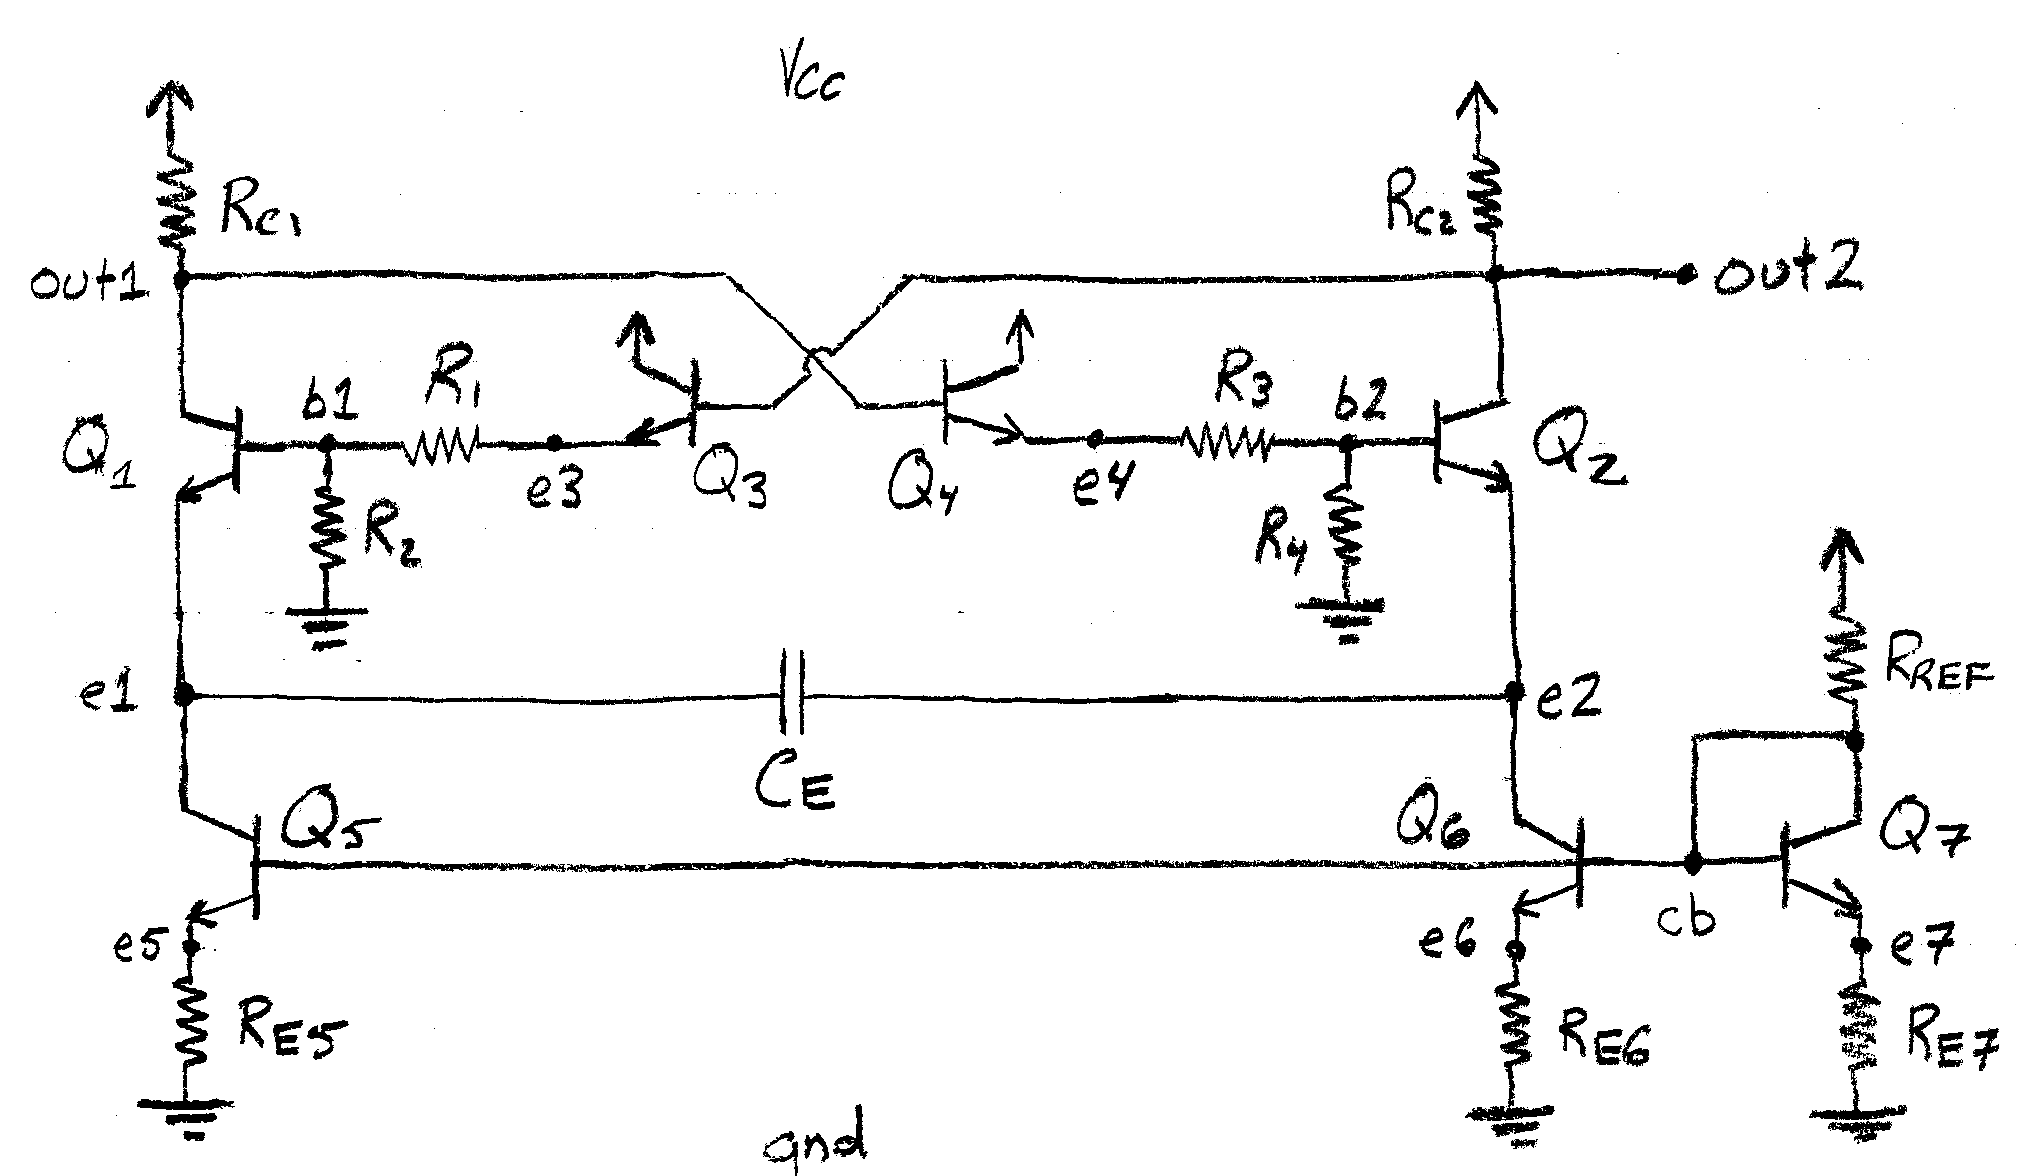
\includegraphics[width=0.8\textwidth]{diagrams/advanced-circuit}
	\caption{Advanced Version of Astable Multivibrator}
	\label{advanced-circuit}
\end{figure}

The two switching transistors are still labeled $Q_{1}$ and $Q_{2}$.
Transistors $Q_{3}$ and $Q_{4}$ are emitter-folowers that provided more current
to the cross connections.
These voltage buffers are an inprovement because $R_{1}$ and $R_{2}$ can be reduced
to inprove the charging time of the parasitic base-emitter junction capacities.

Transistors $Q_{5-7}$ are set up as current mirrors to provide constant current
to both of the switching transistors. This is an inprovment because limiting the
current with the resistors has unwanted effects on the voltages the cause switching.
Additionally, in the simple circuit, the emitter resistors had to be large enough
to handle significant power.

The current from the mirrors
should be equal to the average transistor current, or half of the
saturation current because only one switching transistor is on at any moment.
\begin{equation*}
I_{mirror}=I_{C(ave)}
\end{equation*}

For a current mirror, the emitter resistors should be equal and small and
the current will be set by the saturation current through $R_{REF}$.
\begin{equation}
I_{mirror}=\frac{V_{CC}-V_{BE(on)}}{R_{REF}+R_{E7}}
\quad \textrm{or} \quad
R_{REF}=\frac{V_{CC}-V_{BE(on)}}{I_{C(ave)}}-R_{E7}
\label{advanced-rref-eq}
\end{equation}

After setting up the current mirrors, they can be ignored and replaced
by constant current sources. See figure \ref{advanced-circuit-without-mirrors}.

\begin{figure}[ht]
	\centering
	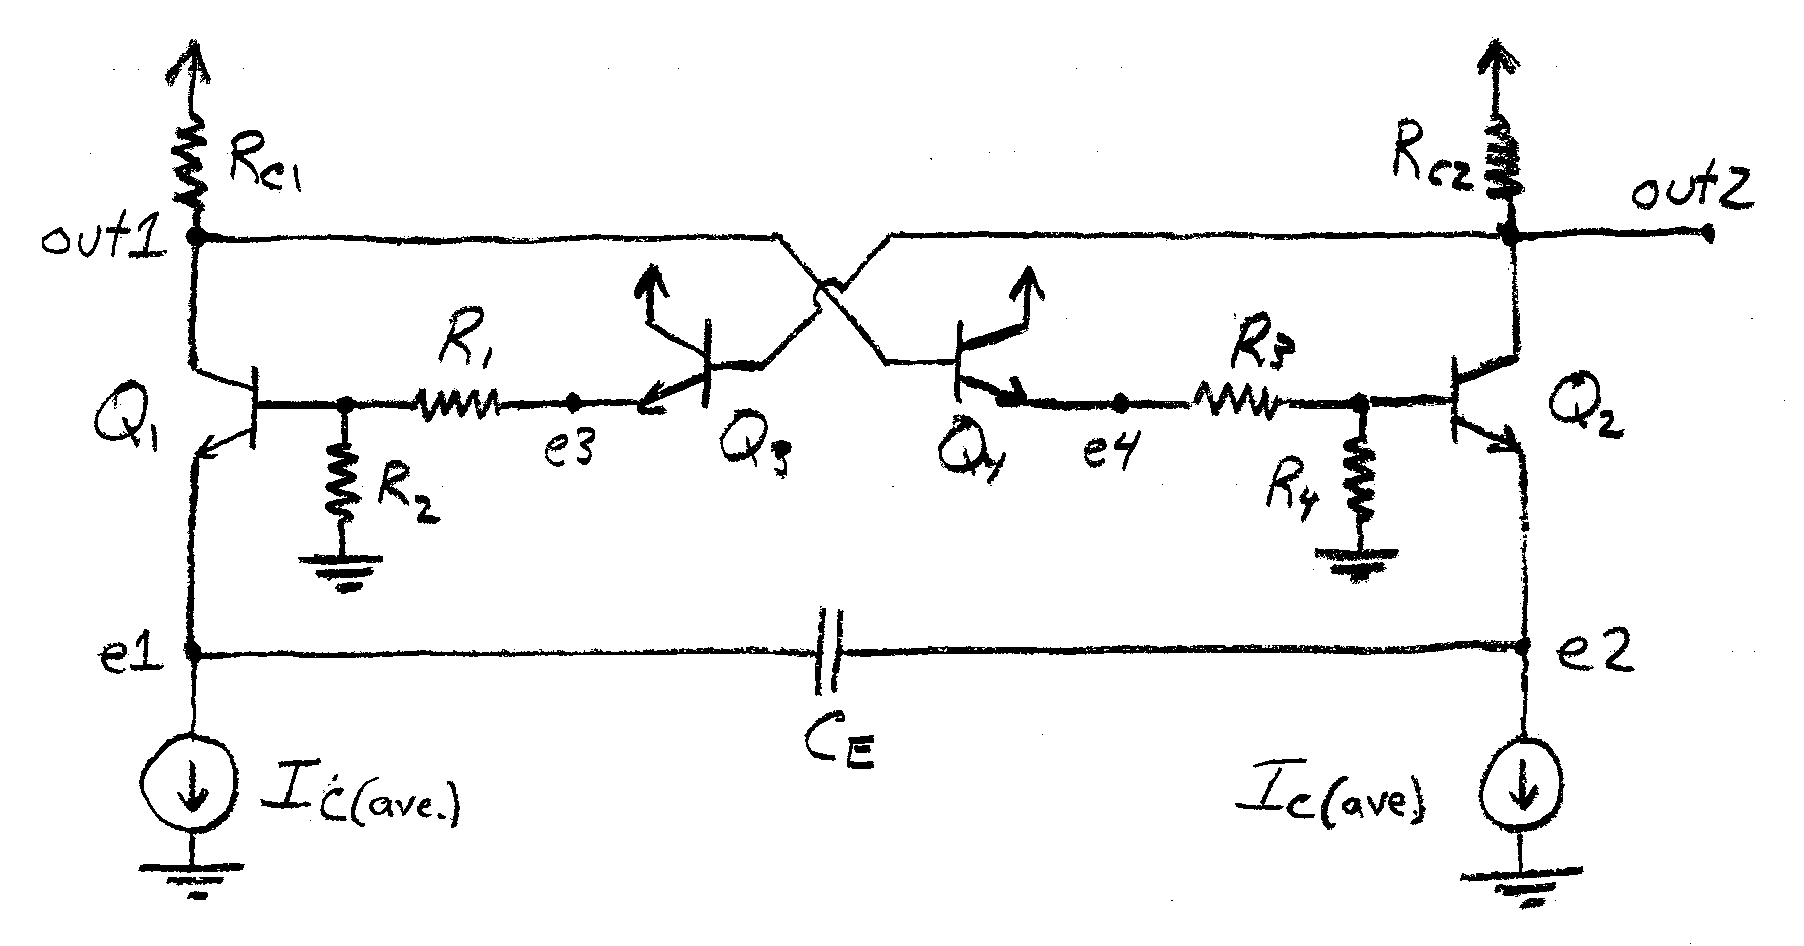
\includegraphics[width=0.8\textwidth]{diagrams/advanced-circuit-without-mirrors}
	\caption{Advanced Circuit with Equivalent Current Sources}
	\label{advanced-circuit-without-mirrors}
\end{figure}

The amplitude of the output swing and the current from the current mirrors are related by $R_{C}$.
\begin{equation}
I_{C(sat)}=2*I_{C(ave)}
\end{equation}
\begin{equation}
R_{C}=\frac{V_{pkpk}}{I_{C(sat)}}
\label{advanced-rc-eq}
\end{equation}

The inputs for $Q_{1}$ and $Q_{2}$ come from the output state of the opposited transistor,
after passing through the voltage buffer and a voltage divider.
\begin{equation*}
\left\{\begin{array}{lr}
V_{B(sat)}=\frac{R_{2}}{R_{1}+R_{2}}(V_{CC}-V_{BE(on)})	\\
V_{B(off)}=\frac{R_{2}}{R_{1}+R_{2}}(V_{CC}-V_{pkpk}-V_{BE(on)})
\end{array}\right.
\end{equation*}

The current state of the switching transistors is stable as long as
the potential at the emitter of the off transistor is withing 0.7 V of
that transistor's base. The on transistor would remain on indefinitely
if the off transistor did not abruptly change the base biasings.
\begin{equation}
\left\{\begin{array}{lr}
V_{E(sat)}=\frac{R_{2}}{R_{1}+R_{2}}(V_{CC}-V_{BE(on)})-V_{BE(on)}	\\
V_{E(off)}>\frac{R_{2}}{R_{1}+R_{2}}(V_{CC}-V_{pkpk}-V_{BE(on)})-V_{BE(on)}
\end{array}\right.
\label{advanced-stability-conditions}
\end{equation}

The top half of the circuit has now been analyzed and equation
\ref{advanced-stability-conditions} provide the stability conditions for
which we can treat the top half as a black box. To analyze the transient
bottom half of the circuit, the top half can be replaced by ideal switches
connected to the emitter voltage at saturation from first stability condition.
This simplified circuit will remain valid until the emitter voltage at the off
switch violates the second stability condition.
\begin{equation}
V_{E(trig)}=\textrm{Min}(V_{E(off)})=\frac{R_{2}}{R_{1}+R_{2}}(V_{CC}-V_{pkpk}-V_{BE(on)})-V_{BE(on)}
\end{equation}

The equivalent circuit for the transient analysis is shown in figure
\ref{advanced-transient-circuit}.

\begin{figure}[ht]
	\centering
	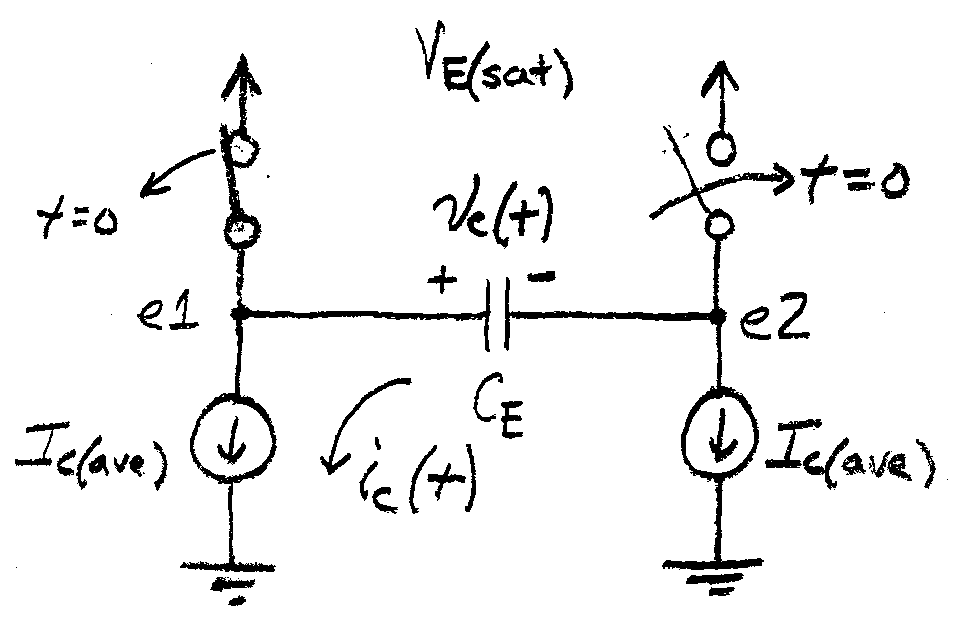
\includegraphics[width=0.45\textwidth]{diagrams/advanced-transient-circuit}
	\caption{Transient Model for the Advanced Astable Multivibrator}
	\label{advanced-transient-circuit}
\end{figure}

At the instant before switching occurs, $v_{e1}$ is shorted to $V_{E(sat)}$ and
$v_{e2}$ is approaching $V_{E(trig)}$. So,
\begin{equation}
v_{c}(0^{-})=V_{E(sat)}-V_{E(trig)}
\label{advanced-initial-condition}
\end{equation}

The current through the capacitor is fixed by the constant current source
of the off transistor's side.
\begin{equation*}
i_{C}(t)=I_{C(ave)}
\end{equation*}

Replacing the capacitor current with the capacitor i-v relationship yields
a first order, separable differential equation.
\begin{equation*}
-C_{E}\frac{dv_{E}}{dt}=I_{C(ave)}
\end{equation*}

Solving gives an equation for voltage across the capacitor.
\begin{equation*}
dv_{C}=\frac{-I_{C(ave)}}{C_{E}}dt
\end{equation*}

\begin{equation*}
\int 1*dv_{C}=\frac{-I_{C(ave)}}{C_{E}}\int 1*dt
\end{equation*}

\begin{equation*}
v_{C}(t)=\frac{-I_{C(ave)}}{C_{E}}t+K
\end{equation*}

The constant from integration should be the initial voltage across the capacitor.
Substituting this in from equation \ref{advanced-initial-condition} gives
\begin{equation}
v_{C}(t)=\frac{-I_{C(ave)}}{C_{E}}t+V_{E(sat)}-V_{E(trig)}
\end{equation}

The voltage across the capacitor is directly related to the off emitter voltage.
We are interested in the period of time for which the off emitter voltage is greater
than the trigger voltage.
\begin{equation*}
v_{E(off)}=V_{E(sat)}+v_{C}(t)
\end{equation*}

\begin{equation*}
v_{E(off)}=V_{E(sat)}+\frac{-I_{C(ave)}}{C_{E}}t+V_{E(sat)}-V_{E(trig)}
\end{equation*}

\begin{equation*}
V_{E(trig)}=V_{E(sat)}+\frac{-I_{C(ave)}}{C_{E}}T_{stable}+V_{E(sat)}-V_{E(trig)}
\end{equation*}

\begin{equation}
T_{stable}=\frac{2C_{E(trig)}(V_{E(sat)}-V_{E(trig)})}{I_{C(ave)}}
\end{equation}

The period of stability for one transistor is half of the square wave cycle,
so the frequency of oscillation is defined by
\begin{equation}
f=\frac{I_{C(ave)}}{4C_{E}[V_{E(sat)}-V_{E(trig)}]}
\quad, \quad
C_{E}=\frac{I_{C(ave)}}{4f[V_{E(sat)}-V_{E(trig)}]}
\end{equation}

\section{Design and Simulation}

\subsection{Specifications}

For this lab I needed to build a square wave, emitter-coupled oscillator
that meets the specifications in table \ref{specs-table}.

\begin{table}[ht]
\centering
\caption{Emitter-Coupled Oscillator Design Specifications}
\begin{tabular}{c | c | c}
\hline\hline
Parameter	&Notation	&Value	\\
\hline\hline
Power Supply	&$V_{CC}$	&24 V	\\
Output Signal Amplitude	&$V_{pkpk}$	&2 V	\\
Maximum Frequency	&$f$	&50 MHz	\\
Average $I_{C}$ of Switching Transistor	&$\frac{I_{C(sat)}}{2}$	&6 mA	\\
\hline\hline
\end{tabular}
\label{specs-table}
\end{table}

\subsection{BJT Characterization}

\subsection{Simple Circuit Design}

An astable multivibrator was designed with the theory derived in sections
\ref{bistable-latch} and \ref{astable-multivibrator} in order to meet the
specifications for the lab in table \ref{specs-table}.
The circuit diagram is shown again in figure \ref{simple-circuit-2}.

\begin{figure}[ht]
	\centering
	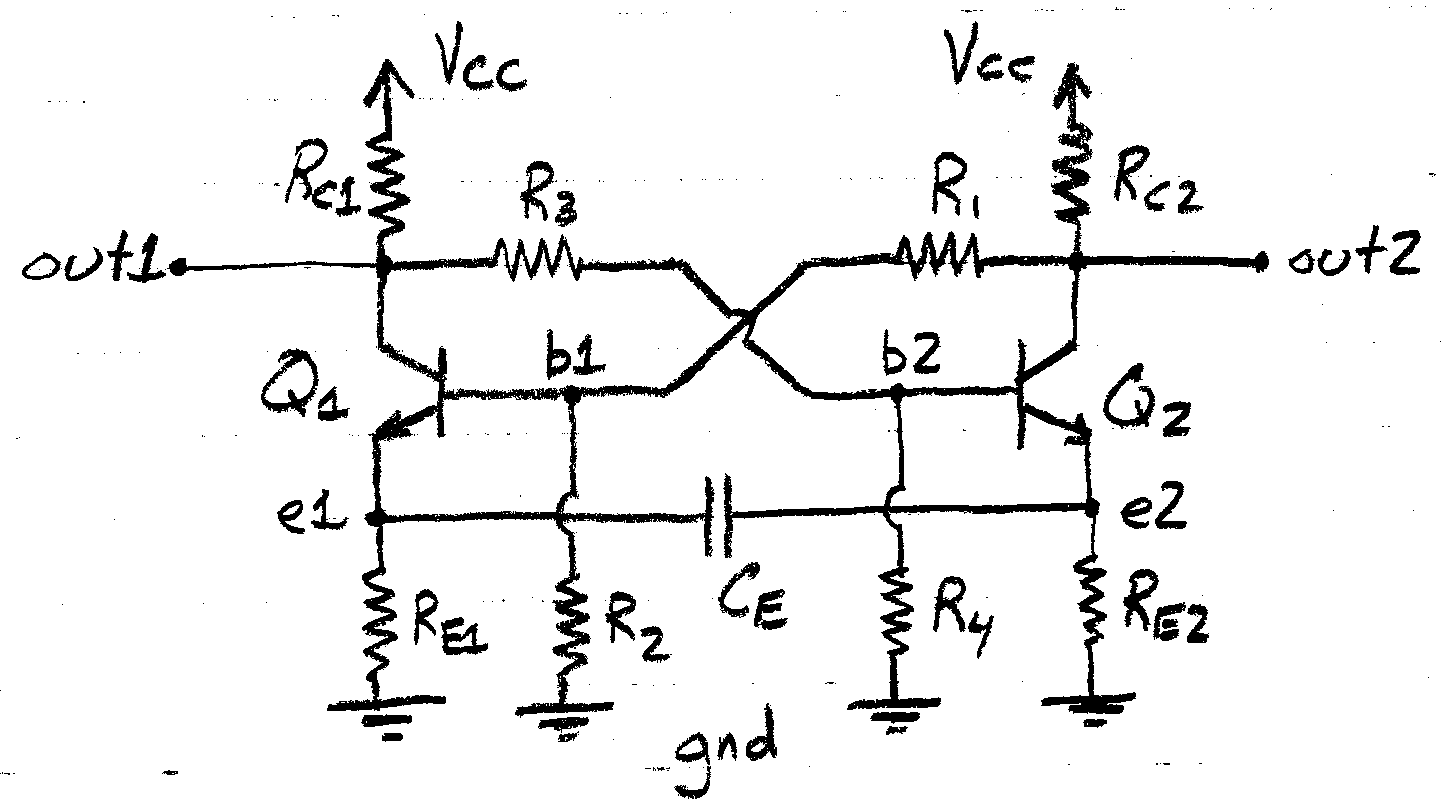
\includegraphics[width=.5\textwidth]{diagrams/simple-circuit}
	\caption{Simple Circuit Diagram}
	\label{simple-circuit-2}
\end{figure}

Table \ref{simple-circuit-design-table} shows the values that were calculated
while designing the circuit and the corresponding equations used.

\begin{table}[ht]
\centering
\caption{Original Simple Circuit Design}
\begin{tabular}{c | c | c}
\hline\hline
Parameter	&Designed Value	&Design Method	\\
\hline\hline
$V_{CC}$	&24 V	&specified	\\
$V_{pkpk}$	&2.4 V	&specified $+20\%$	\\
$I_{C(sat)}$	&12 mA	&$2*I_{C(ave)}$	\\
$R_{1}+R_{2}$	&$20k\Omega$	&equation \ref{r1r2-eq}	\\
$\frac{R_{2}}{R_{1}+R_{2}}$	&0.917	&equation \ref{stability-conditions}	\\
$V_{E(sat)}$	&21.31 V	&equation \ref{ve-sat-eq}	\\
$V_{E(trig)}$	&19.47 V	&equation \ref{ve-trig-eq}	\\
\hline
Component	&Designed Value	&Design Method	\\
\hline
$R_{C}$	&$200\Omega$	&equation \ref{rc-eq}	\\
$R_{2}$	&$18.3k\Omega$	&$R_{2}=\frac{R_{2}}{R_{1}+R_{2}}(R_{1}+R_{2})$	\\
$R_{1}$	&$1.7k\Omega$	&$R_{1}=(R_{1}+R_{2})-R_{2}$	\\
$R_{E}$	&$1.7k\Omega$	&equation \ref{re-eq}	\\
$C_{E(0.1MHz)}$	&17,000 pF	&equation \ref{ce-eq}	\\
$C_{E(1MHz)}$	&1,700 pF	&equation \ref{ce-eq}	\\
$C_{E(10MHz)}$	&170 pF	&equation \ref{ce-eq}	\\
$C_{E(50MHz)}$	&17 pF	&equation \ref{ce-eq}	\\
\hline\hline
\end{tabular}
\label{simple-circuit-design-table}
\end{table}

When the simple circuit was built according to the original design in table
\ref{simple-circuit-design-table},
square wave oscillations were observed but the higher frequencies could not be achieved.
The most likely cause of this limitation was the delay time associated with charging the
parasitic base-emitter junction capacities. Charge has to flow through $R_{1}$ and collect
on the base for some time.
A quick, back-of-the-hand calculation with the junction capacities in table \ref{bjt-characterization-table}
shows this is on the order of 10 ns.
\begin{equation*}
\tau=R_{1}C_{JE}=8.9ns\quad\quad f=111MHz
\end{equation*}


\subsection{Simple Circuit Redesign}

\subsection{Simple Circuit SPICE Simulation}

\subsection{Advanced Circuit Design}

\subsection{Advanced Circuit SPICE Simulation}

\section{Results}
\end{document}
